\subsection{OpenStack background}

\subsubsection{Swift}

Swift is a highly available, distributed, eventually consistent object storage which can operate standalone or integrated with the rest of the OpenStack cloud computing platform. It is used  to store lots of data efficiently, safely, and cheaply using a scalable redundant storage system \cite{swift-definition}. As opposed to conventional storage architectures like file systems which manage data using file hierarchy and block storage, Swift manages data as objects. Each object typically includes the data itself, a variable amount of metadata, and a globally unique identifier.

%\textbf{Swift Servers}: 
Using its well defined RESTful API \cite{swift-api}, users can upload or download objects to and from Swift storage. Inside Swift, objects are organized into containers which is similar to directories in a filesystem except that Swift containers cannot be nested. Again, a user is associated with a Swift account and can have multiple containers associated with the account. In order to manage user accounts, user containers and objects inside a container, Swift uses an Account Server, a Container Server and Object Servers correspondingly.

When a user corresponding to a user account requests for an object inside a container (either for uploading or downloading), the Account Server looks for the account first in its account database and finds associated containers with the account. The Container Server then checks the container database to find whether the requested object exists in the specified container and finally the Object Server looks into `object databases' to find retrieval information about the object. In order to retrieve an object, the Proxy Server needs to know which of the Object Servers are storing the object, and path of the object in the local filesystem of that server.



% For interacting with objects stored inside Swift storage, it provides a RESTful API using HTTP request methods (e.g. GET, PUT, DELETE etc).


\subsubsection{Swift ACL}
	Once an object is stored in Swift, who can or cannot access the object is determined by Swift Access Control List (ACL).  Swift has  different levels of ACL---Account level ACL, and Container level ACL, for example. Container level ACL is associated with containers in term of a \emph{read} action, or \emph{write} action  or \emph{listing} action. If a user is authorized read action on a container through read ACL, he or she can read or download objects from the container. Similarly, write ACL enables uploading an object into a container and listing ACL enables the list operation on the container. Account ACLs, on the other hand, allow users to grant account-level access to other users.  Of these two types of ACL, Container level ACL is  finer grained in that different containers of a single account can be configured differently. Nonetheless, Swift ACL is limited in the following ways.
	
\begin{itemize}
	\item  Once an object is set accessible  to someone, he or she gets the full content of the object. But  there can be some sensitive information that the publisher wants to hide out.
		
	 \item  Swift ACL allows  sharing an object with others, but it does not allow to share objects selectively at the content level.
	
\end{itemize}	
%--------------Following section is commented---------------------
%Account level ACL is specified in terms  of  \emph{read-only}, \emph{read-write} and \emph{admin} operation. For example, anyone having \emph{read-only} ACL on the account level can do a listing on all the containers or read all objects of all containers associated with the Account.
%Using ACL, it is possible to specify who can access objects inside the container. Examples of some supported ACLs are `read' ACL, `write' ACL, `listing' ACL and so on. With Swift ACL, we can either specify a positive list and a negative list. For example, a read acl with following ACL value \emph{ `.referrer:*'} allows everyone to read or download objects from corresponding container.  On the other hand, value of \emph{`.referrer:*-example.com} as read ACL, remove read permission for request coming from example.com as a referrer.

%A point to note is that Swift ACL either allows and denies access to an object. Once  ACL allows access to an object, the requester gets full content of the object. So, essentially, ACL based access is an `all or nothing' approach and cannot be used to share a Swift object selectively among different users.

%--------------commenting ends here---------------------


%\subsection{JSON (JavaScript Object Notation)}

%JSON or JavaScript Object Notation is a data representation format which uses human readable text to represent data. In JSON, data is represented in one of two forms---as an \emph{object} or as an \emph{array of values}. A JSON object is defined as a collection of \emph {key-value} or \emph {attribute-value} pairs where a \emph {key} or an \emph {attribute}\footnote{To avoid confusion with the use of \emph{attribute} for attribute-based access control we will exclusively use the term \emph{key} in this paper.} is simply a string representing a name  and a \emph {value} which is either one of the following primitive types---string, number, boolean (true or false), null or another object or an array. On the other hand, an array is defined as a set of an ordered collection of \emph {values} (as defined above) starting from index zero. The formal definition of JSON data format is given in   \cite{json-official-website}. JSON structure has following characteristics

%\begin{enumerate}
%  \item A JSON document forms a hierarchical structure which is a rooted tree.
%  \item In the rooted tree, leaf nodes represent text data of the document and non-leaf nodes are used to give the data a name and thus  organize it.
%  \item In the rooted tree, a node can be uniquely identified by traversing the document from the root node to the target node.
%\end{enumerate}



%JSON or JavaScript Object Notation is a data representation format which uses human readable text to represent data. In JSON, data is represented in one of two forms -  as an object or as an array of values. In our implementation, we use a JSON object or a JSON array as the minimum protection unit and assign object-label values on them. Figure \ref{fig:labelled-json-data} shows a sample JSON document with its objects being labelled as `personal', `public', `protected' and so on. In simple situations, roles of a user can be used as his user-label values. A simple policy for the given JSON data is \emph{ (`personal', read, `patient')} which means that JSON objects labelled with `personal' can only be read by users having a label of `patient'.


\begin{figure}
  \centering
    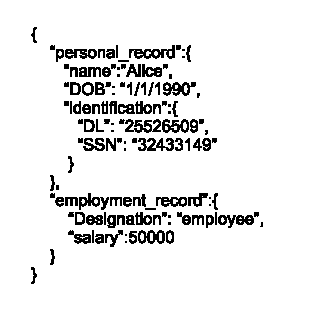
\includegraphics[width=0.3\textwidth]{CODASPY15/json-data}
 \caption{A sample JSON Document containing   records of an employee.}
   \label{fig:json-data}
\end{figure}



\subsection{Label Based Access Control}
In order to protect a JSON document stored as a Swift object, we assign each JSON item (i.e. value of a JSON key) an \emph{object-label} and each user a \emph{user-label}. Then we specify policies  in the form of  (\emph{user-label} values, \emph{action},  \emph{object-label} values)   which means that objects labeled with any of `object-label' values are allowed to be accessed by the users labeled with any of  `user-label' values for the specific `action'. Here we present an informal description of the model and its open source implementation is available in \cite{labac}.

\begin{figure*}
\centering
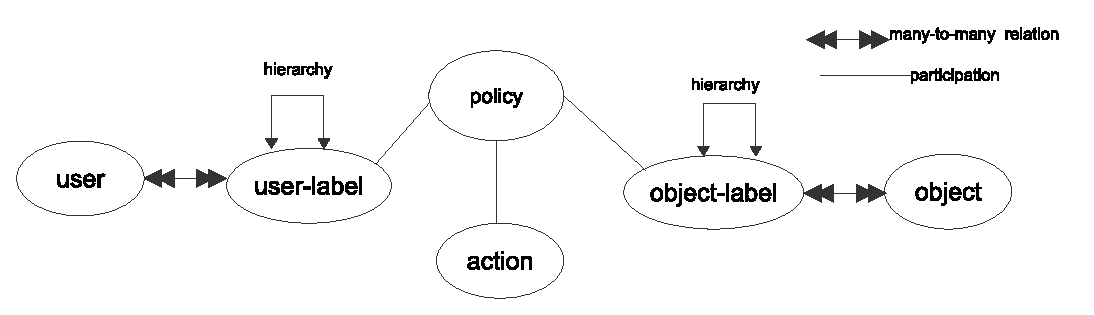
\epsfig{file=CODASPY15/labac-model.eps}
\caption{Label Based Access Control Model.}
\label{fig:labac-model}
\end{figure*}


\subsubsection{Model Components}

In LaBAC (Figure \ref{fig:labac-model}), we have one attribute assigned to objects and one attribute assigned to users. Object attribute is named  \emph{object-label} and user attribute is named \emph{user-label}. These attributes are set valued attributes and the values of the attributes may form a partial order.
%Note that, both object-label and user-label are a special type of attribute  which we do not elaborate here for brevity.

\emph{Object}: Object is any resource we want to protect with the model. Examples include a JSON document or items inside a JSON document. 

\emph{Object-label}: Object-label is the attribute assigned on the objects. The values of this attribute  may form a partial order.

\emph{User} and \emph{user-label}: User-label is the attribute assigned on each user. In a simple case, user-label values can be the set of roles assigned to the user. The values of this attribute may form a partial order.

\emph{Action}: Action is the list of available actions to be exercised on the objects. 
%Although, it is possible to have hierarchy on action, to keep the model simple we do not introduce action hierarchy.

\emph{Policy}: A policy in this model is a tuple of (\emph{user-label} values, \emph{action},  \emph{object-label} values). The policy is interpreted such that objects labeled with any of `object-label' values are allowed to be accessed by the users labeled with any of  `user-label' values for the specific `action'.

\emph{Attribute Hierarchy}: In our model, both object-label and user-label values  may form a hierarchy or more specifically a partial order. The effect of attribute hierarchy is shown in Figure \ref{fig:attribute-hierarchy}. As we can see in the figure, if a policy allows an action for user-label $l_{uj}$ on object-label $l_{oj}$, due to the attribute hierarchy, all users having a equivalent or senior label than $l_{uj}$ can also access object-label $l_{oj}$ or its junior labels.

\begin{figure}
  \centering
    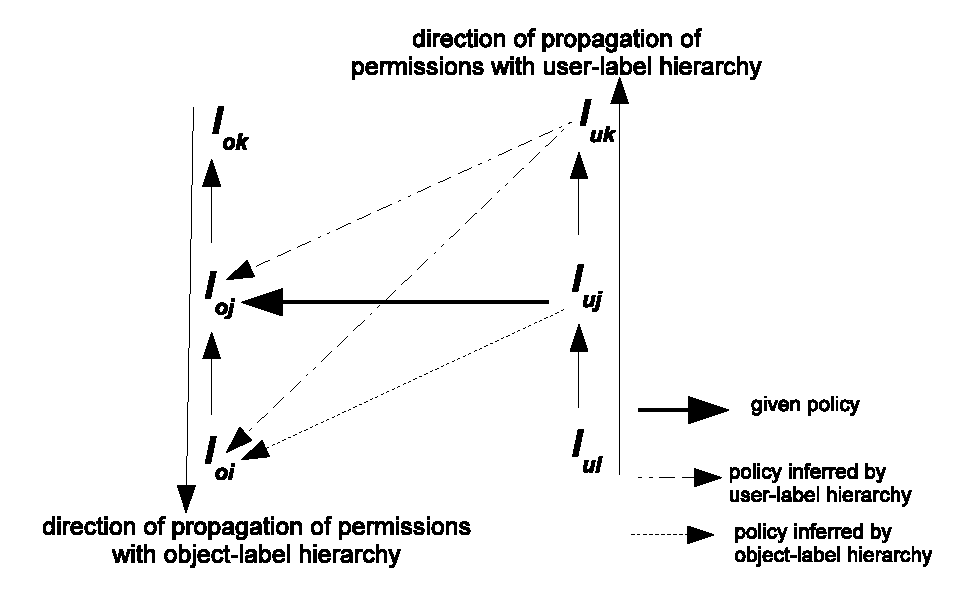
\includegraphics[width=0.5\textwidth]{CODASPY15/attribute-hierarchy}
 \caption{Propagation of permission with attribute hierarchy.}
 \label{fig:attribute-hierarchy}
\end{figure}

 \subsection{Content Level Protection}


Swift ACL specifies who can or cannot access a Swift object but it cannot   specify who can access which part of the object.  In order to specify security policies at the content level, Swift has to be aware of the content type and data format of the object. In our case, we addressed Swift objects of content-type \emph{`application/json'} which is  standard JSON format. How our protection mechanism works  is summarized below.

\begin{itemize}
\item JSON items to be protected are identified using JSONPath. For example, SSN in JSON data given in Fig. \ref{fig:json-data} is identified using JSONPath `\$.personal\_record.ide ntification.SSN'.
\item  \emph{object-label} values are assigned on the specified JSON item. For example, to specify that SSN is a sensitive information, we assign a label \emph{`sensitive'} on JSONPath `\$.personal\_record.identification.SSN'.

\item We use LaBAC policy to specify who can access (read) which \emph{object-label}. For example, if only users with user-label `manager' can access \emph{sensitive} information, then we specify the LaBAC policy \emph{(`manager', read, `sensitive')}.

\end{itemize}

When using JSONPath to identify a JSON item, one may want to  specify value at the path  as a condition. For example, salary information (given in Fig. \ref{fig:json-data}) is sensitive only if the salary is greater than 50,000. Furthermore, it is also possible to protect one item based on value of a different item. For example, identification information (specified by JSONPath   `\$.personal\_record.identification') of a user is sensitive when his salary is greater than 50,000.

\subsection{Labeling  JSON Items}
If the JSON document is large, labeling all JSON items can be tedious. In order to reduce labeling effort, we propagate label assigned on a JSON item to all its descendant items. For example, if the \emph{personal\_record}  item (Fig. \ref{fig:json-data}) is labeled \emph{sensitive}, then all its descendant nodes (name, DOB, identification, DL, SSN) are also labeled  \emph{sensitive}.



